\begin{figure}[H]
  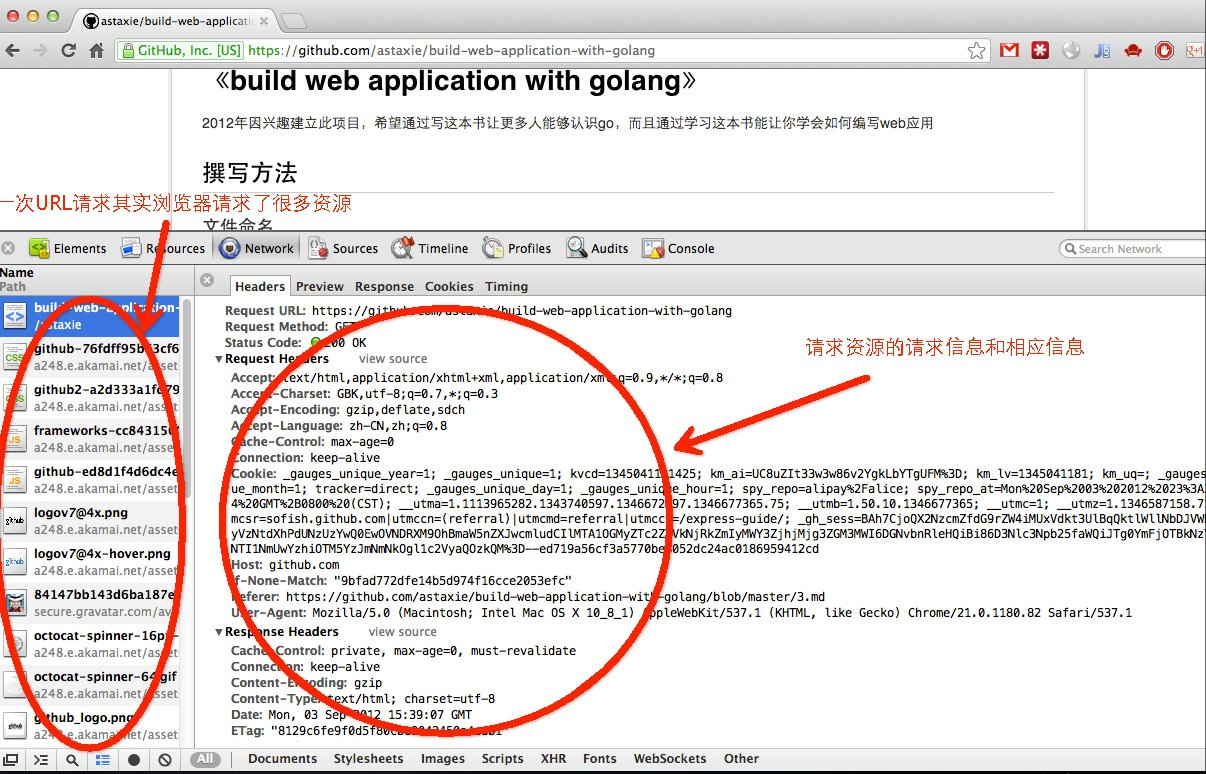
\includegraphics[width=14cm]{3.1.web.jpg}
   \label{図3.7}
   \caption{一回の要求のrequestとresponse}
\end{figure}



上の図で全体の通信プロセスをご理解いただけるかと思います。同時に注意深い読者はひとつのURLリクエストにもかかわらず左のペインではどうしてこのように多くのリソース要求があるのかと思われたかもしれません。(これらはすべて静的なファイルです。goは静的なファイルに対して専門的に処理する方法を有しています。)

これはブラウザの機能の一つです。URLを一度要求すると、サーバはhtmlページを返します。その後ブラウザはHTMLを読み取り、HTMLのDOMの中にあるイメージリンク、cssスクリプトとjsスクリプトのリンクを見つけた時、ブラウザは自動的に静的なリソースのHTTP要求を行います。目的の静的なリソースを取得すると、ブラウザは読み始めます。最後にすべてのリソースを整理し、我々の前のスクリーン上に展開します。

\begin{quote}
ホームページの改良では、HTTPのリクエスト回数を減らすことがあります。つまり、なるべく多くのcssとjsリソースを同じところに集めるのです。目的は出来る限りホームページの静的リソースのリクエスト回数を減少させる事にあります。ホームページの表示速度を上げると同時にサーバのバッファリングを減らす事ができます。
\end{quote}
